\section{Background and The Algorithm}
\label{section:algorithm}
Please present the essential background knowledge and the algorithm in this section. You may also describe the notations and the optimization problem of interest.

\subsection{Problem Formulation}
\begin{itemize}
\item POMDP

%POMDP
As mentioned in section \ref{section:intro}, this paper models the market as partially observable Markov decision process (POMDP) instead of traditional Markov decision process(MDP) due to the noisy trading environment. We can't exactly know what the current market state is, and the only thing we can know is its partial observation.

$$
\text{POMDP}
\left\{
\begin{aligned}
&\left.
\begin{aligned}
&S : \text{a finite set of states} \\
&A : \text{a finite set of actions} \\
&T : S*A*S \rightarrow [0,1] : \text{a state transition function} \\
&R : S*A \rightarrow R : \text{a reward function} \\
&\gamma : \text{a discount factor} \\
\end{aligned}
\right\} \text{MDP}\\
&O : \text{the corresponding observations of $S$} \\
&Z : S*A*O \rightarrow [0,1] : \text{the corresponding observation transition function of $T$}
\end{aligned}
\right.
$$

\item Observation
%%Observation

The observation $O$ we can get involves historical price $\mathbb{P}$, various technical indicators $\mathbb{Q}$, and account profit, $\mathbb{R}$. The transition function of the whole observation set can fit the POMDP framework $Z=Z(o_{t+1}|s_{t+1},a_t)$. But trading actions from an individual investor have little impact on the entire market which means $Z=Z(o^m_{t+1}|s_{t+1})$, hence the whole observation set of POMDP separates the first two parts as the market observation $O^m$ from the last part as the account observation $O^a$. Except for the original market observation in this paper, we also add some additional variables into $O^m$ like moving average, margin, stochastic oscillator (KD) to increase the convergence process. Note that the account profit is just a observation, not the reward.

$$
O
\left\{
\begin{aligned}
&\left.
\begin{aligned}
\mathbb{P} &: [p_1,...,p_t,...], \text{ and }\mathbb{P}_{t-n:t} = [p_{t-n+1},...,p_{t-1},p_t], \\
&\quad  \text{ where } p_t=[p^o_t, p^h_t, p^l_t, p^c_t], \text{ an open,high,low,close price vector}\\
\mathbb{Q} &: [q_1,...,q_t,...], \text{ where } q_t = \cup_j q_t^j,  \text{ an indicator vector},\\
&\quad q_t^j=f(\mathbb{P}_{t-n:t};\theta^j), \text{ and }\theta^j \text{ is parameter of technical strategy }j 
\end{aligned}
\right\}O^m\\
&\left.\mathbb{R} : [r_1,...,r_t,...], \text{ where $r_t$ is the account profit}\right\}O^a \\
\end{aligned}\right.
$$

$$
\begin{aligned}
\Rightarrow & o^a_t \in O^a, \text{ where } o^a_t \text{ denotes the cumulative account profit, } \sum_{k=1}^t r_k \in \mathbb{R}\\
&o^m_t \in O^m, \text{ where } o^m_t \text{ is related with $p_t$ and $q_t$}
\end{aligned}
$$

\item Action
%Action

The trading action $a_t$ is defined as a continuous probability vector, and the final executed action will be the one with maximal probability. Furthermore, it doesn't mean that the agent should always place an new order to change the position based on the executed action. A new position will be placed or be changed only if the current executed action is empty or alternate from long/short to short/long.
$$
a_t = [P_{long}, P_{short}]
$$

\item Reward
%Reward

Account profit $r_t \in \mathbb{R}$ includes two transaction factors, transaction fee $\delta$ and slippage $\zeta$.
$$
r_t = (p_t^c-p_{t-1}^c-2\zeta)a_{t-1} - \delta|a_t-a_{t-1}|p_t^c
$$
It's not appropriate to use it as reward, because the account profit will often be zero and sparse as the new order not being placed. Instead, this paper uses differential sharp ratio (DSR) $D_t$ as the reward function $R$. It is the dynamic version of sharp ratio $Sr_t$ that can measure the return while considering the risk.
$$
\begin{aligned}
Sr_t &= \frac{E[\mathbb{R}_{t-n:t}]}{\sigma [\mathbb{R}_{t-n:t}]},\\
D_t
&\equiv \frac{dSr_t}{d\eta}
=\frac{\beta_{t-1}\Delta \alpha_t-\frac{1}{2}\alpha_{t-1}\Delta \beta_t}{(\beta_{t-1}-\alpha^2_{t-1})^{3/2}},\\
\text{ where } \eta& \text{ is the adaptation rate},\\
\alpha_t &\text{ and $\beta_t$} \text{ are exponential moving estimates of first and second moment of $r_t$,}\\ \alpha_t &= \alpha_{t-1} + \eta \Delta \alpha_t = \alpha_{t-1}+\eta(r_t-\alpha_{t-1}),\\
\beta_t &= \beta_{t-1}+\eta \Delta \beta_t = \beta_{t-1} + \eta(r^2_t - \beta_{t-1}).
\end{aligned}
$$
\end{itemize}


\subsection{Methodology--RDPG}
Memory-based control with recurrent neural networks (\cite{heess2015memory}) try to improve DDPG by introducing the recurrent neural networks. The method proposed is called Recurrent Deterministic Policy Gradient abbreviate as RDPG.

DDPG is an actor-critic approach, which bridges the gap between policy gradient methods and value approximation methods for RL.
The agent trains the critic network by minimizing the TD error.
Simultaneously, the agent learns a deterministic policy actor by directly maximizing the estimated Q function from critic.

This paper use of the GRU to effectively synthesize historical information.
The objective function and optimization method for RDPG are almost the same to DDPG. 
However, because the RDPG will be updated through BPTT, so the unit of an experience in the replay buffer is a sequence data, not a step data .

We show the RDPG algorithm bellow:

\begin{small}
\quad\quad

\quad\quad Initialize critic network $Q^{\omega}\left(a_{t}, h_{t}\right)$ and actor $\mu^{\theta}\left(h_{t}\right)$ with parameters $\omega$ and $\theta$. 

\quad\quad Initialize target networks $Q^{\omega^{\prime}}$ and $\mu^{\theta^{\prime}}$ with weights $\omega^{\prime} \leftarrow \omega, \theta^{\prime} \leftarrow \theta$.

\quad\quad Initialize replay buffer $R$. 

\quad\quad for episodes $=1, \mathrm{M}$ 

\quad\quad\quad\quad do initialize empty history $h_{0}$ 

\quad\quad\quad\quad for $\mathrm{t}=1, \mathrm{~T}$ do receive observation $o_{t}$

\quad\quad\quad\quad\quad\quad $h_{t}=G R U\left(h_{t-1}, a_{t-1}, o_{t}\right)($ append      

\quad\quad\quad\quad\quad\quad observation and previous action to history $)$ 

\quad\quad\quad\quad\quad\quad select action $a_{t}=\mu^{\theta}\left(h_{t}\right)+\epsilon($ with $\epsilon:$ exploration noise $)$ 
    
\quad\quad\quad\quad end for 
    
\quad\quad\quad\quad Store the sequence $\left(o_{1}, a_{1}, r_{1} \ldots o_{T}, a_{T}, r_{T}\right)$ in $R$ 
    
\quad\quad\quad\quad Sample a minibatch of $N$ episodes $\left(o_{1}^{i}, a_{1}^{i}, r_{1}^{i}, \ldots o_{T}^{i}, a_{T}^{i}, r_{T}^{i}\right)_{i=1, \ldots, N}$ from $R$
    
\quad\quad\quad\quad Construct histories $h_{t}^{i}=\left(o_{1}^{i}, a_{1}^{i}, \ldots a_{t-1}^{i}, o_{t}^{i}\right)$
    
\quad\quad\quad\quad Compute target values for each sample episode $\left(y_{1}^{i}, \ldots y_{T}^{i}\right)$ using the recurrent target networks
$$
y_{t}^{i}=r_{t}^{i}+\gamma Q^{\omega^{\prime}}\left(h_{t+1}^{i}, \mu^{\theta^{\prime}}\left(h_{t+1}^{i}\right)\right)
$$
    
\quad\quad\quad\quad Compute critic update (using BPTT)
$$
\text { loss } L=\mathbb{E}\left[\left(y_{t}^{i}-Q^{\omega}\left(h_{t}^{i}, a_{t}^{i}\right)\right)^{2}\right]
$$
    
\quad\quad\quad\quad Compute actor update (using BPTT)
$$
\nabla_{\theta} J=\mathbb{E}\left[\left.\left.\nabla_{a} Q^{\omega}(h, a)\right|_{h=h_{t}^{i}, a=\mu^{\theta}\left(h_{t}^{i}\right)} \nabla_{\theta} \mu^{\theta}(h)\right|_{h=h_{t}^{i}}\right]
$$
    
\quad\quad\quad\quad Update actor and critic using Adam Update the target networks
$$
    \begin{array}{r}
    \omega^{\prime} \leftarrow \tau \omega+(1-\tau) \omega^{\prime} \\
    \theta^{\prime} \leftarrow \tau \theta+(1-\tau) \theta^{\prime}
    \end{array}
$$
\quad\quad end for
\end{small}


\subsection{Methodology--Demonstration Buffer}
In order to enhance the effectiveness of training, \cite{liu2020adaptive} introduced the imitation learning technique.
Since the detail is limited in previous paper, we refer to the practice in DDPGfD (\cite{vecerik2017leveraging}) to implement demonstration buffer. As the name suggests, demonstration buffer will store expert Demonstration first. The expert policy is from Dual Thrust strategy which will be explained later.

To enable efficient propagation of the reward information they apply prioritized expereince replay(PER) (\cite{schaul2015prioritized}).
In PER, The probability of sampling a particular transition $i$ is proportional to its priority, $P(i)=\frac{p_{i}^{\alpha}}{\sum_{k} p_{k}^{\alpha}}$,  where $\alpha$ is hyperparameter and $p_{i}$ is the priority of the transition.
DDPGfD uses $p_{i}=\delta_{i}^{2}+\lambda_{3}\left|\nabla_{a} Q\left(s_{i}, a_{i} \mid \theta^{Q}\right)\right|^{2}+\epsilon+\epsilon_{D}$, where $\delta_{i}$ is the last TD error calculated for this transition, the second term represents the loss applied to the actor, $\epsilon$ is a small positive constant to ensure all transitions are sampled with some probability, $\epsilon_{D}$ is a positive constant for demonstration transitions to increase their probability of getting sampled, and $\lambda_{3}$ is used to weight the contributions. To account for the change in the distribution, updates to the network are weighted with importance sampling weights, $w_{i}=\left(\frac{1}{N} \cdot \frac{1}{P(i)}\right)^{\beta}$. $\beta$ is hyperparameter.


\subsection{Methodology--Behavior Cloning}
Behavior cloning is try to clone the expert policy.
In hindsight, we can create a prophetic trading expert.
That is, we introduce intra-day greedy actions as expert actions. 
As shown by the picture, we take a long position at lowest price, and a short position at highest price. Therefore, it is always a relatively optimal greedy strategy.

\begin{figure}[h!]
    \center
    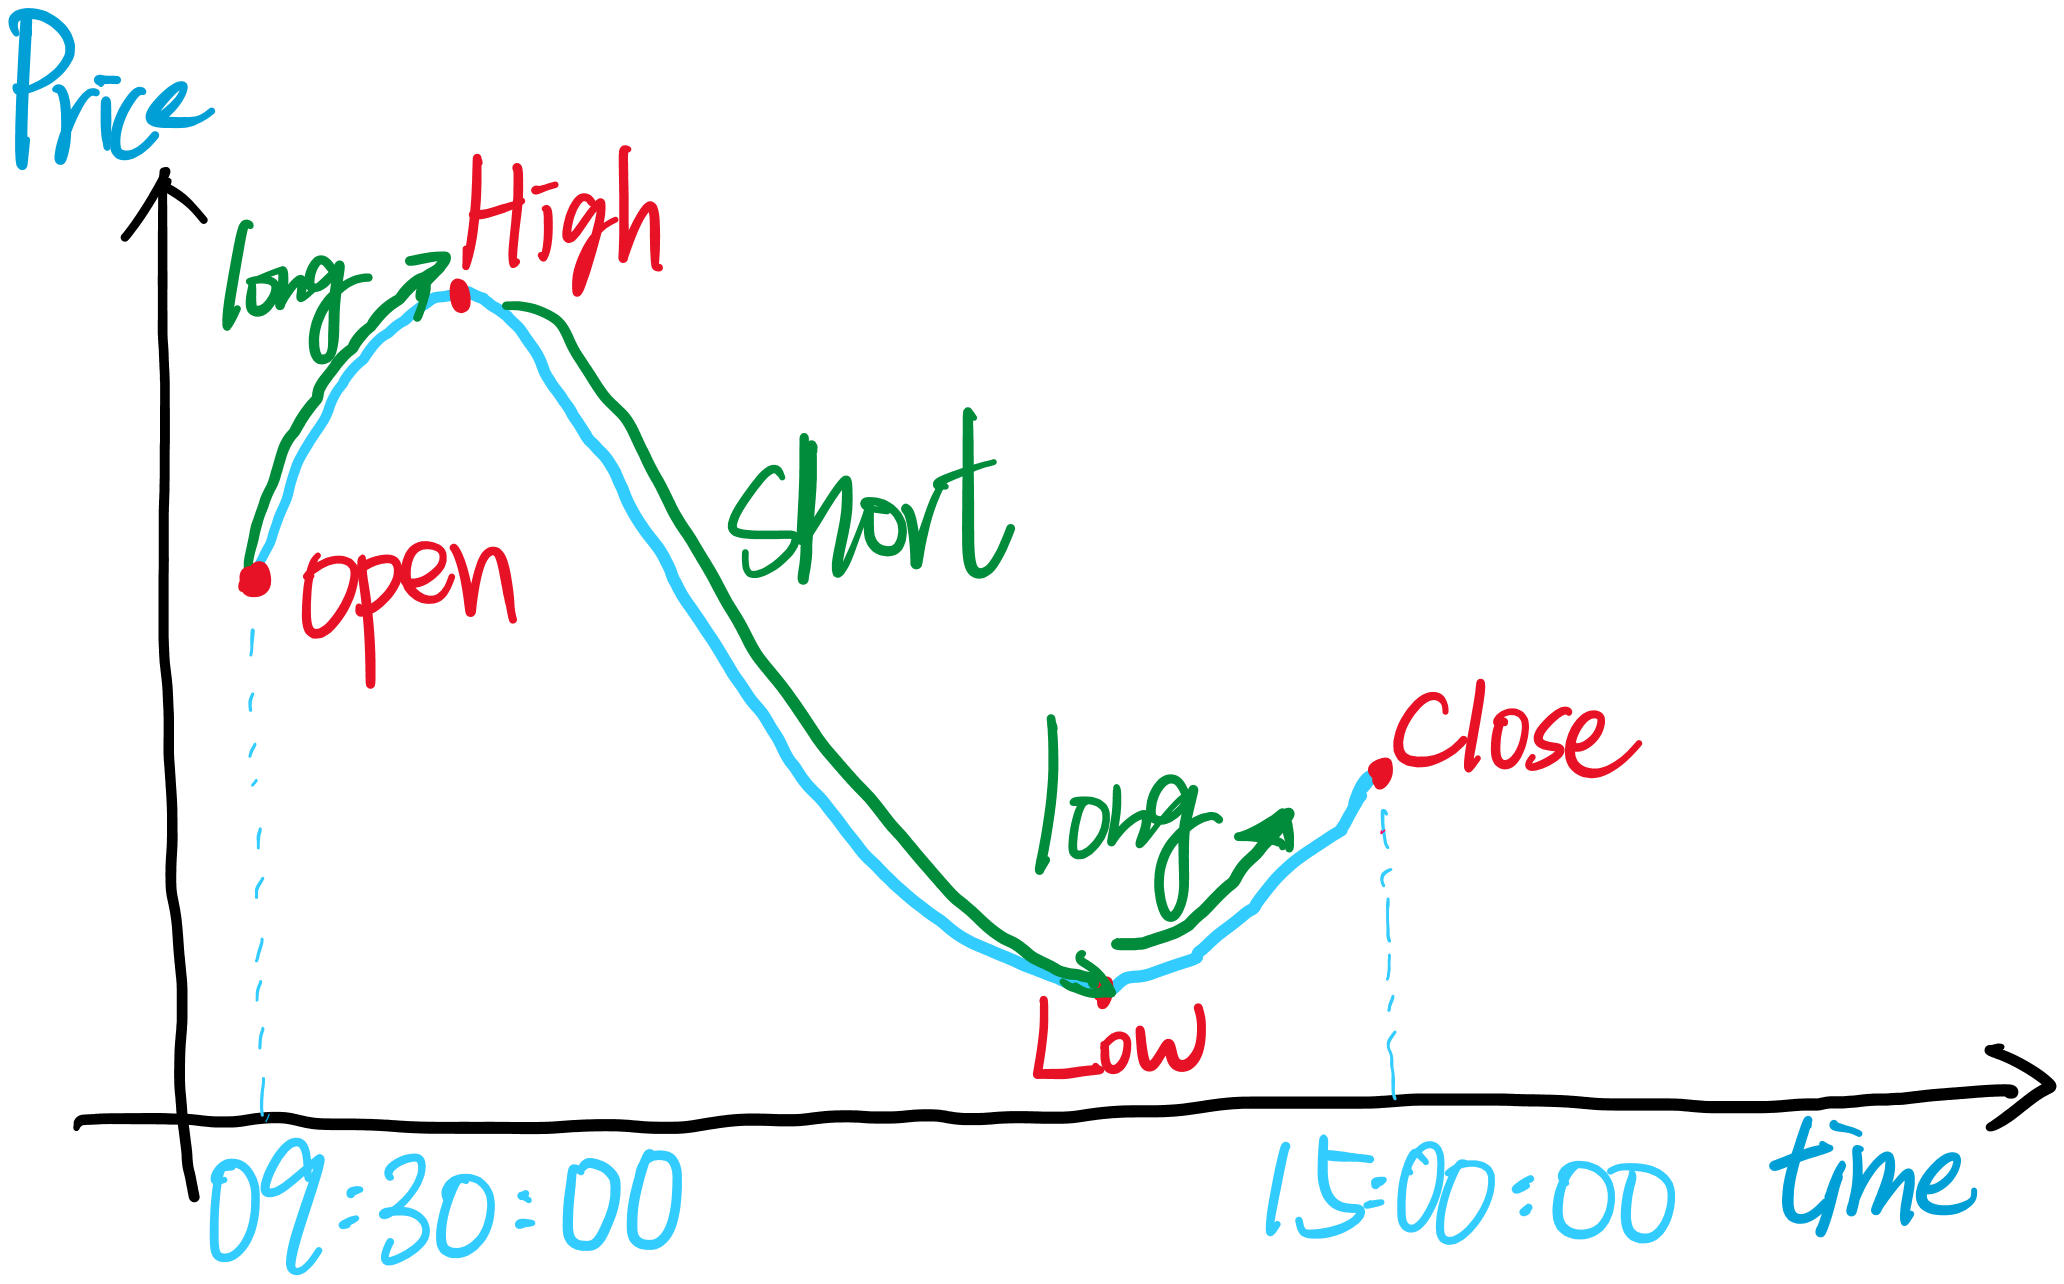
\includegraphics[width=8cm]
    {BC_demo3}
    \caption{  intra-day greedy actions as expert actions }
    \label{fig:  Using intra-day greedy actions as expert actions }
\end{figure}

The next is about the loss function. You could see the down figure.
Since Behavior cloning is a kind of supervised learning approach, we take the square of the policy difference between actor and expert. \\
In addition, we apply the Q-filter technique.
That is, we record BC Losses only when the critic Q indicates that the expert actions perform better than the actor action.\\
Finally, as shown by the picture below, we combine the BC loss with the original objective function, and calculate its policy gradient for updating the actor.


\begin{figure}[h!]
    \center
    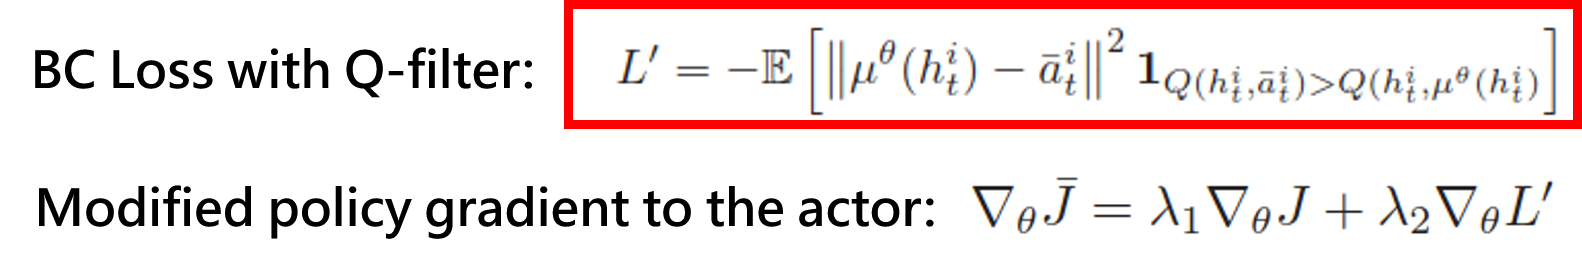
\includegraphics[width=9cm]
    {BC}
    % \caption{ Q-filter and modified policy gradient }
    \label{fig: The IF IC}
\end{figure}



